\documentclass{article}
\usepackage{tikz}
\usetikzlibrary{shapes.geometric, arrows}

\tikzstyle{startstop} = [rectangle, rounded corners, minimum width=3cm, minimum height=1cm,text centered, draw=black]
\tikzstyle{process} = [rectangle, minimum width=3cm, minimum height=1cm, text centered, draw=black]
\tikzstyle{arrow} = [thick,->,>=stealth]

\begin{document}

\begin{center}
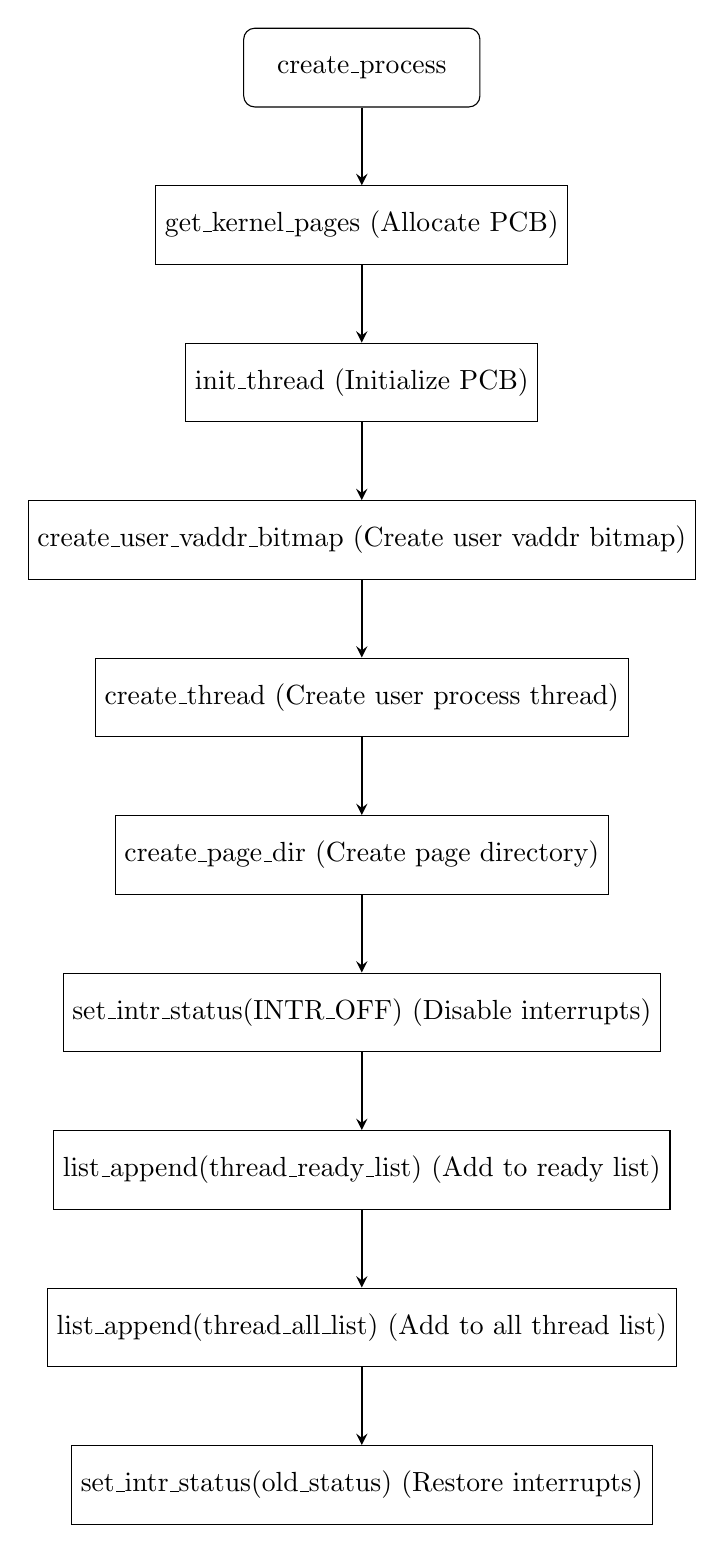
\begin{tikzpicture}[node distance=2cm]

    \node (start) [startstop] {create\_process};
    \node (A) [process, below of=start] {get\_kernel\_pages (Allocate PCB)};
    \node (B) [process, below of=A] {init\_thread (Initialize PCB)};
    \node (C) [process, below of=B] {create\_user\_vaddr\_bitmap (Create user vaddr bitmap)};
    \node (D) [process, below of=C] {create\_thread (Create user process thread)};
    \node (E) [process, below of=D] {create\_page\_dir (Create page directory)};
    \node (F) [process, below of=E] {set\_intr\_status(INTR\_OFF) (Disable interrupts)};
    \node (G) [process, below of=F] {list\_append(thread\_ready\_list) (Add to ready list)};
    \node (H) [process, below of=G] {list\_append(thread\_all\_list) (Add to all thread list)};
    \node (I) [process, below of=H] {set\_intr\_status(old\_status) (Restore interrupts)};

    \draw [arrow] (start) -- (A);
    \draw [arrow] (A) -- (B);
    \draw [arrow] (B) -- (C);
    \draw [arrow] (C) -- (D);
    \draw [arrow] (D) -- (E);
    \draw [arrow] (E) -- (F);
    \draw [arrow] (F) -- (G);
    \draw [arrow] (G) -- (H);
    \draw [arrow] (H) -- (I);

\end{tikzpicture}
\end{center}

\end{document}
